% Generate boilerplate to create a document with a title page, name, date with a report style
% Usage: \report{Title}{Name}{Date}

\documentclass{report}

\usepackage{graphicx}  % For including images
\usepackage{amsmath}   % For mathematical symbols and environments
\usepackage{hyperref}  % For hyperlinks
\usepackage{wrapfig}  % For wrapping text around figures
\usepackage{geometry}  % For setting page dimensions

% Set the margins
\geometry{
    left=0.5in,  % Adjust the left margin
    right=0.5in, % Adjust the right margin
    top=0.5in,   % Adjust the top margin (optional)
    bottom=0.5in % Adjust the bottom margin (optional)
}

% Command to create the title page
\newcommand{\report}[3]{
    \title{#1}
    \author{#2}
    \date{#3}
    \maketitle
}

\begin{document}

% Create the title page
\report{Lyapunov Orbits}{Roberto Lucchesi 1744941}{\today}

\vfill
\begin{center}
    \textit{All code available at:} \url{https://github.com/Meoli96/Trajectory}
\end{center}

\newpage

\section*{Lyapunov Orbits}
Lyapunov orbits are planar symmetric periodic orbits around the collinear points for the 3CRBP.
In order to find such solutions, the Jacobian of the linearized dynamical model around the 
equilibrium point is considered, and through diagonalization, 
two real eigenvalues (one positive $\boldsymbol{E_u}$ and one negative $\boldsymbol{E_s}$) 
and one complex pair $\boldsymbol{E_{c1}}$, $\boldsymbol{E_{c2}}$ is found.\\\\
Periodic motion is possible only in the subspace spanned by the eigenvectors corresponding to the complex eigenvalues.
Deriving the linearized equation of motion in this subspace, the state equation for a Lyapunov orbit is obtained as:
\begin{equation}
    \boldsymbol{x} = \boldsymbol{x_L} + \alpha_0(\cos(\omega t)Re({\boldsymbol{E_{c1}}}) - \sin(\omega t)Im({\boldsymbol{E_{c1}}})
\end{equation}
with $\alpha_0$ the amplitude of the periodic motion, $\omega$ the frequency of the motion, and $\boldsymbol{x_L}$ the equilibrium point.
The linearization will eventually diverge, and the periodic motion will be accurate only for small amplitudes. \\\\
To improve the accuracy of the solution and make possible the computation of a family of periodic orbits, the problem is formulated as a two-point boundary value problem (TPBVP), thanks to the simmetries of the 3CRBP.
A shooting method is then employed to solve the TPBVP, and a first nonlinear Lyapunov orbit is found from the linear guess.\\\\
Once a first solution is found, a continuation method is employed to find a family of periodic orbits. The Pseudo Archlength Continuation (PAC) is used to follow the family of solutions in the solution space. The following pseudocode illustrates the procedure to 
vary the solution step $d s$ to achieve the continuation:
\begin{verbatim}
    if norm(G) > tol:
        ds = ds/1.1
    else:
        ...
        ds = ds*1.2
        if ds > ds_max:
            ds = ds_max
\end{verbatim}
where $G$ is the residual of the PAC, $tol$ is the tolerance, and $ds_{max}$ is the maximum step size.
This method allows for accuracy on the computation by reducing the step size when the residual is too high, but also for efficiency by increasing the step size when the residual is low enough.\\\\

A family of nonlinear Lyapunov orbits is then found around L1 and L2:
% Plot two images on the same line
\begin{figure}[h]
    \centering
    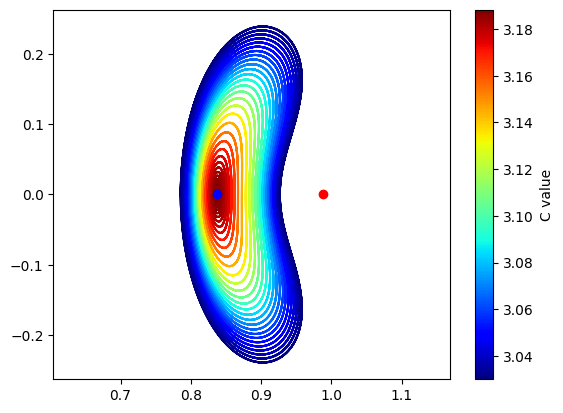
\includegraphics[width=0.49\textwidth]{images/L1.png}
    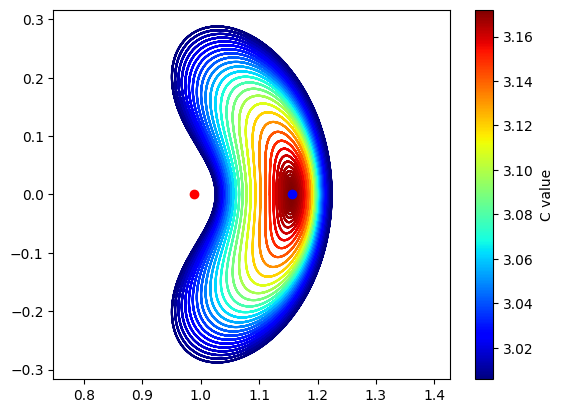
\includegraphics[width=0.49\textwidth]{images/L2.png}
    \caption{Lyapunov orbits around L1 and L2}
\end{figure}
\subsection*{Isoenergetic Lyapunov orbits}
As per request, two pair of isoenergetic Lyapunov orbits is seeked. Two orbits in the Jacobi range
$C_J = [3.1370, 3.1493]$ are found in the family around L1 from the previously computed family. 
A bisection method on the solution step $ds$ is employed to find the two pairs. The following pseudocode illustrates the procedure:
\begin{verbatim}
    ds_a = 0
    ds_b = next_orb_ds
    while abs(C_J - C_J_target) > tol:
        ... # Compute nonlinear Lyapunov orbit with ds_guess
        if C_J > C_J_target:
            ds_a = ds_guess
        else:
            ds_b = ds_guess
        ds_guess = (ds_a + ds_b)/2
   
\end{verbatim}
\begin{figure}[h]
    \centering
    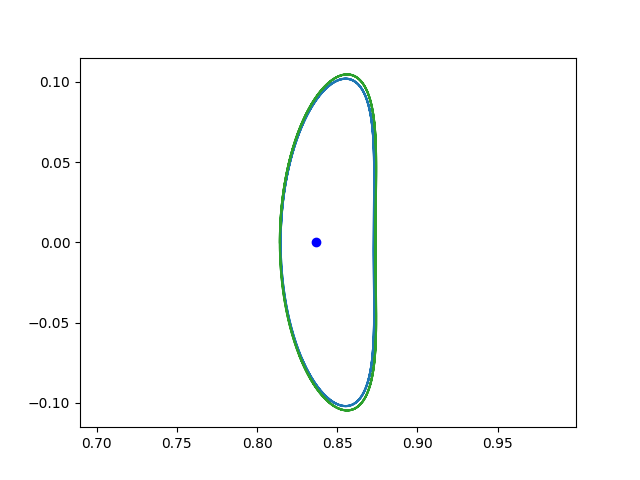
\includegraphics[width=0.49\textwidth]{images/isoL1.png}
    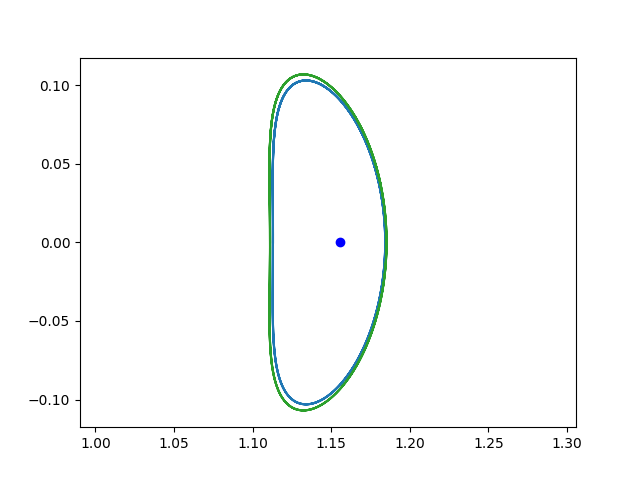
\includegraphics[width=0.49\textwidth]{images/isoL2.png}
    \caption{Isoenergetic Lyapunov orbits}
\end{figure}
In this way two pairs of isoenergetic orbits are found,
with a Jacobi constant of $C_J = 3.1443$ for the first pair and $C_J = 3.1422$ for the second pair.\\\\

\section*{Manifolds}
Manifolds can be computed by perturbing a generic point on the Lyapunov orbit in the stable or unstable subspace
spanned by their respective eigenvector. Letting $\boldsymbol{p}$ be the generic point on the Lyapunov orbit, the perturbation is computed as:
\begin{equation}
    \boldsymbol{x} = p \pm \epsilon \frac{\boldsymbol{E}}{||\boldsymbol{E}||}
\end{equation}
with $\epsilon$ the perturbation, and $\boldsymbol{E}$ the stable or unstable eigenvector\\\\
Manifolds provide an useful insight on the movement of matter of the system, and can be used to compute low-DV transfers between Lyapunov orbits or regions in space.
In particular, stable manifolds will asimptotically approach the Lyapunov orbit, while unstable manifolds will asimptotically diverge from it.
\begin{figure}[h]
    \centering
    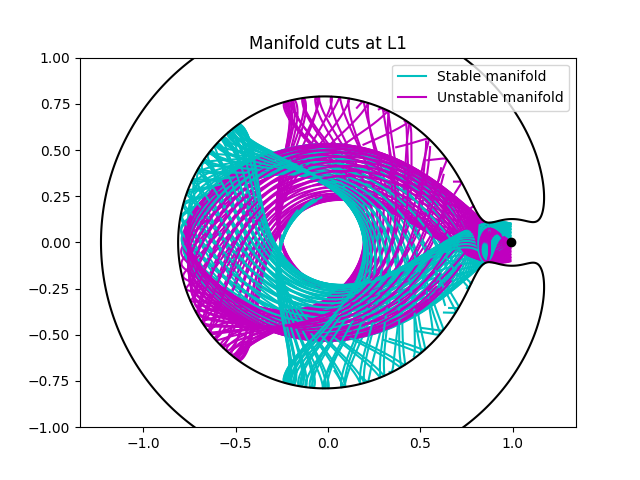
\includegraphics[width=0.49\textwidth]{images/manifold_L1.png}
    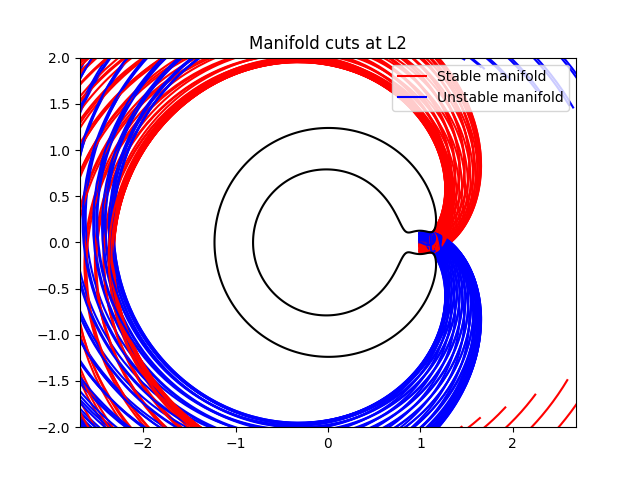
\includegraphics[width=0.49\textwidth]{images/manifold_L2.png}
    \caption{Manifolds around L1 and L2, stable (red) and unstable (blue)}
\end{figure}
\\\\
With the task to compute trajectories, three regions in space are identified:
\begin{itemize}
    \item The Earth region \textbf{E}, inside the ZVC
    \item The Moon region \textbf{M}, inside the ZVC
    \item The outer space region \textbf{X}, outside the ZVC
\end{itemize}
With the use of Poincarè sections, state cuts can be computed to find the initial state to propagate the desired itinerary.
Two of such sections are defined as:
\begin{equation}
    \Sigma_1 : \{x = 1-mu\} \quad \quad \quad \Sigma_2 : \{y = 0\}
\end{equation}
\newpage
\subsection*{[X M E] itinerary}
In order to explore the [X M E] itinerary, the stable manifold of L1 and unstable manifold of L2 are computed, 
divided by the Poincarè section $\Sigma_1$, and the state value at the section are found. 
\begin{figure}[h]
    \centering
    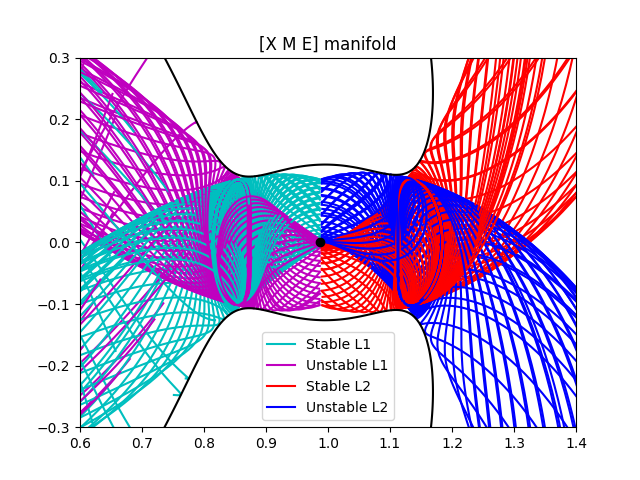
\includegraphics[width=0.49\textwidth]{images/manifold_XME.png}
    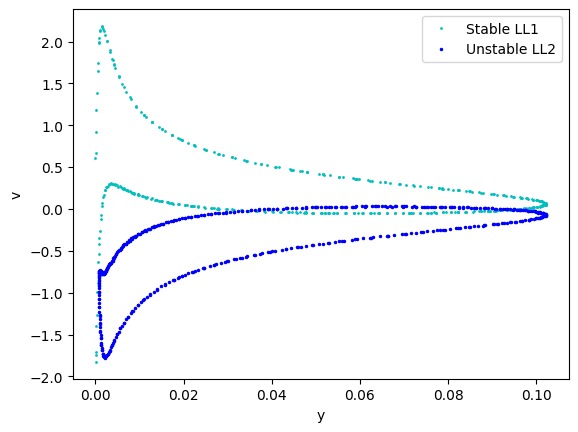
\includegraphics[width=0.49\textwidth]{images/XME_yv.png}
    \caption{Stable L1 and unstable L2}
\end{figure}
By choosing one initial state between the two in the hodograph plane and propagate it backward and forward in time, 
a [X M E] itinerary is found. Due to the problem symmetry, an [X E M] itinerary is also found by inverting the y-u components of the same initial state.
\begin{figure*}[h]
    \centering
    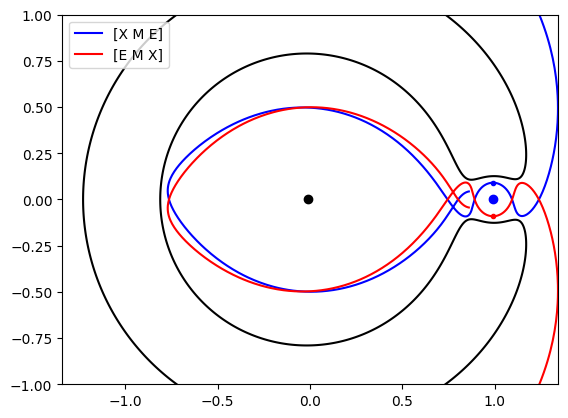
\includegraphics[width=0.5\textwidth]{images/XME_traj.png}
    \caption{[X M E] and [E M X] itineraries}
\end{figure*}
\newpage
\subsection*{[E M E] itinerary}
To plan an [E M E] itinerary the stable and unstable manifolds of L1 are computed, with the Poincarè section $\Sigma_2$.
\begin{figure}[h]
    \centering
    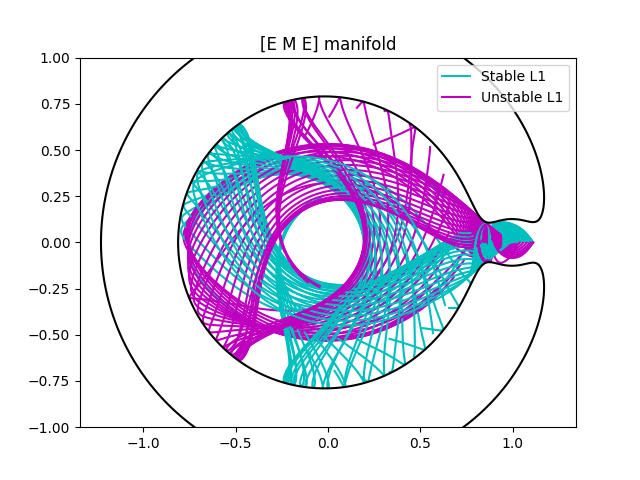
\includegraphics[width=0.49\textwidth]{images/manifold_EME.png}
    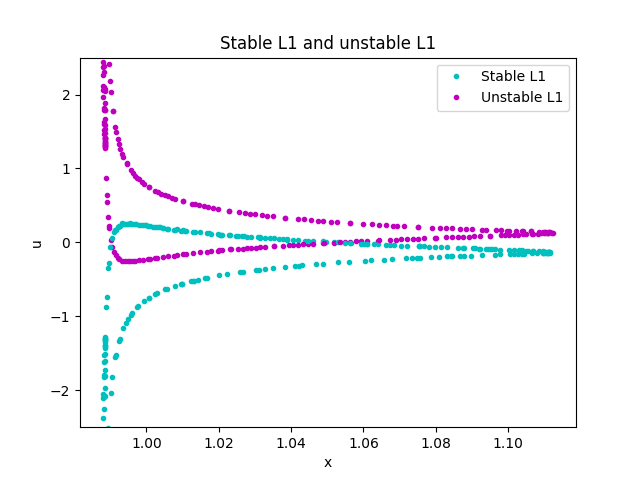
\includegraphics[width=0.49\textwidth]{images/EME_xu.png}
    \caption{Stable and unstable L1}
\end{figure}\\
With the same methodology as before, we compute a trajectory that goes from the Earth to the Moon and back to the Earth.
\begin{figure*}[h]
    \centering
    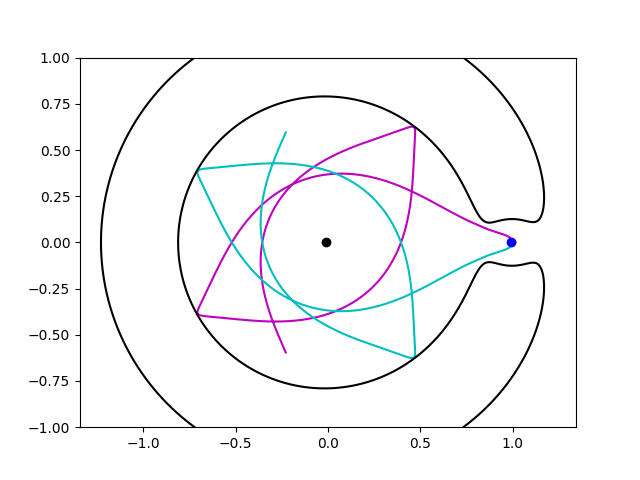
\includegraphics[width=0.49\textwidth]{images/EME_traj.png}
    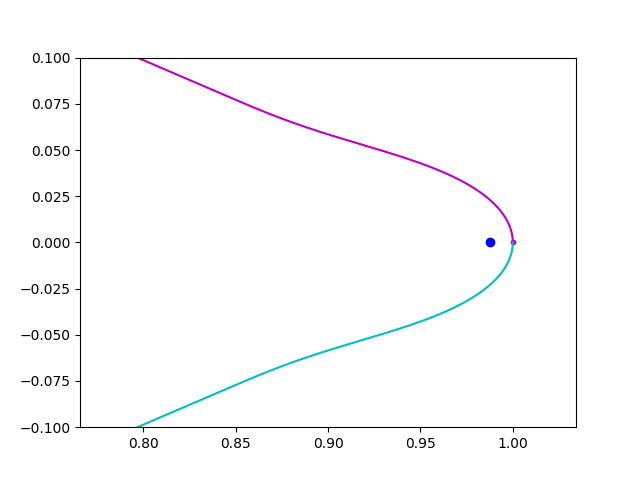
\includegraphics[width=0.49\textwidth]{images/EME_traj_z.png}
    \caption{[E M E] itinerary}
\end{figure*}
\newpage
\subsection*{[X M X] itinerary}
Finally, to plan an [X M X] itinerary, the stable and unstable manifolds of L2 are considered, with the Poincarè section $\Sigma_2$.
\begin{figure}[h]
    \centering
    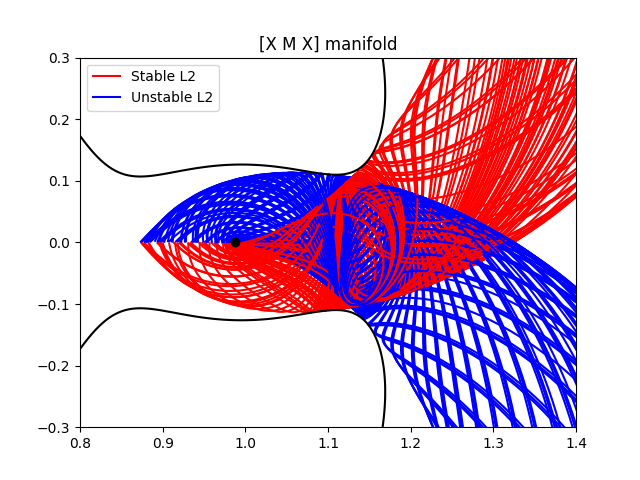
\includegraphics[width=0.49\textwidth]{images/manifold_XMX.png}
    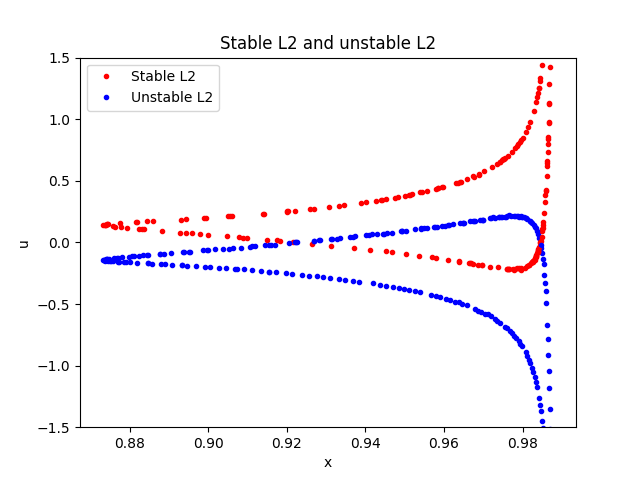
\includegraphics[width=0.49\textwidth]{images/XMX_xu.png}
    \caption{Stable and unstable L2}
\end{figure}
The trajectory is computed as before, and the [X M X] itinerary is found.
\begin{figure*}[h]
    \centering
    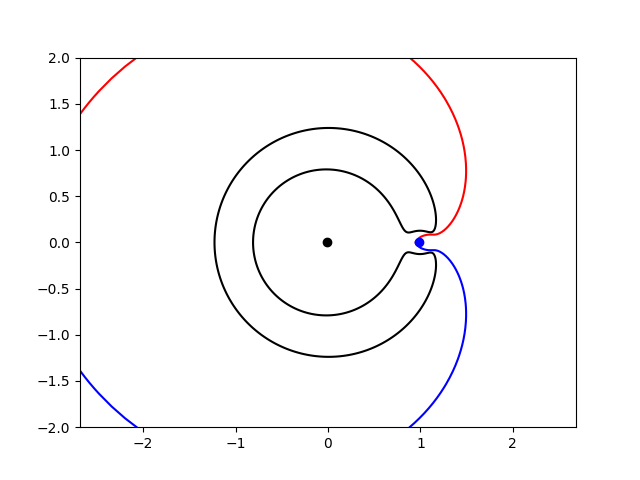
\includegraphics[width=0.49\textwidth]{images/XMX_traj.png}
    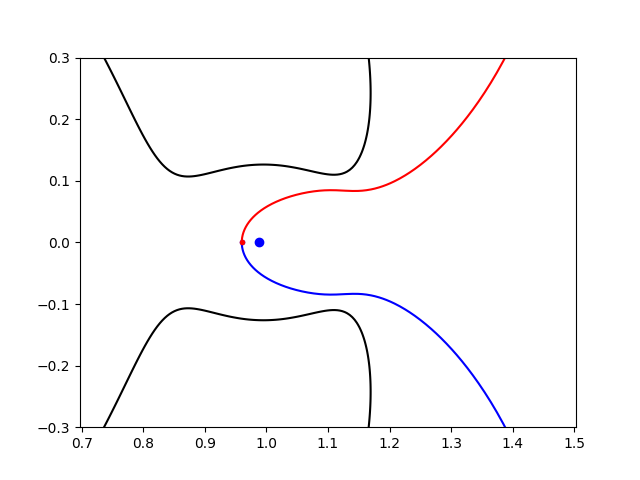
\includegraphics[width=0.49\textwidth]{images/XMX_traj_z.png}
    \caption{[X M X] itinerary}
\end{figure*}



\end{document}